\section{Procedimiento} 

Primeramente crearemos una base de datos llamada BDTEST.Abrir el SQL Server Data Tools y dirigirnos a la pestaña de Business Intelligence -> Analysis Services. Como se creará un Modelo Multidimensional desde 0 , seleccionaremos la primera opción. En la casilla de Name le colocamos un nombre al proyecto y a la solución:
	\begin{center}
	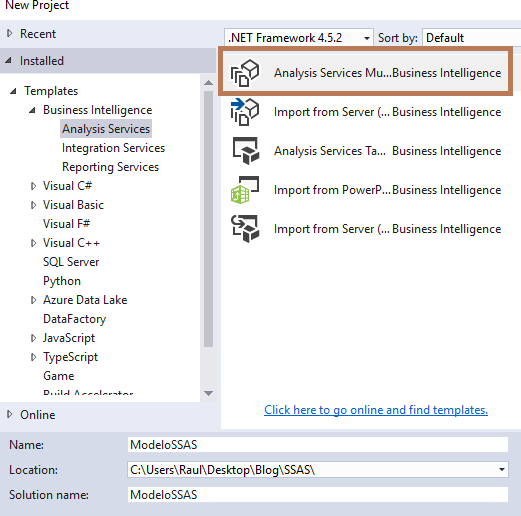
\includegraphics[width=\columnwidth]{images/task1/1}
	\end{center}	

\section{ACTIVIDAD 01 Creación de un Data Source}

En el Solution Explorer nos ubicamos en Data Sources y click derecho, seleccionando la opción de New Data Source
	\begin{center}
	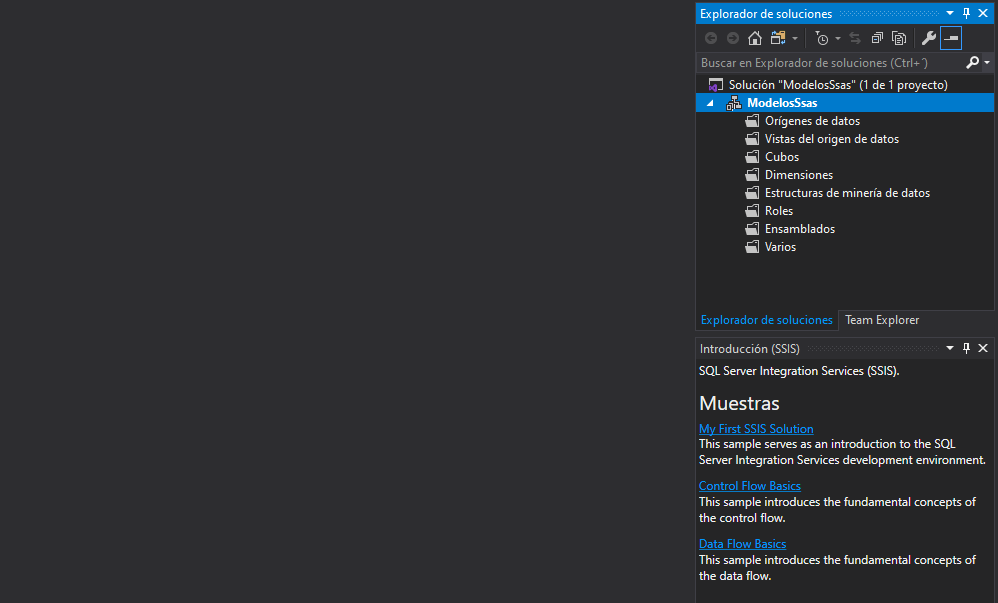
\includegraphics[width=\columnwidth]{images/task1/2}
	\end{center}	

Se nos abrirá una ventana de resumen. Click en Next:
	\begin{center}
	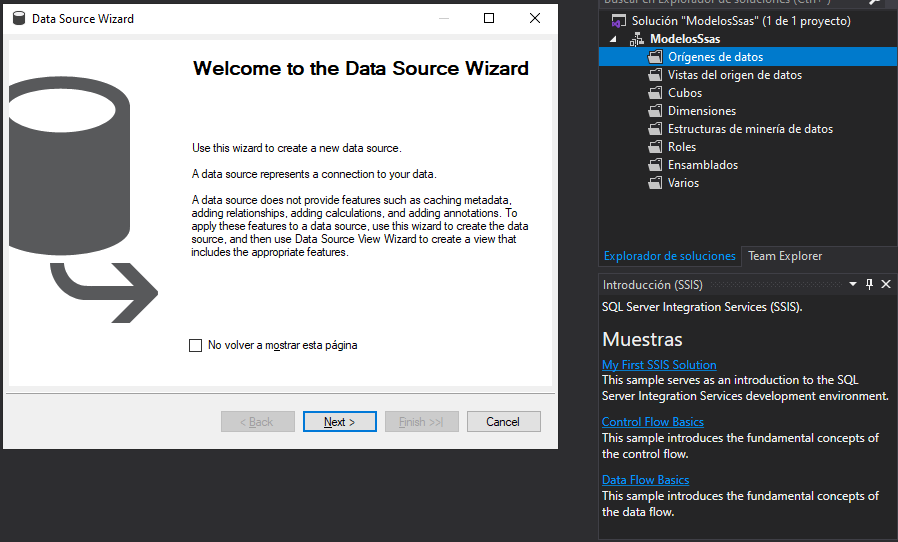
\includegraphics[width=\columnwidth]{images/task1/3}
	\end{center}	

Colocamos el nombre del Server donde se ubica la base de datos, en mi caso como es local coloco “.” , indicándole que es localhost. Ingresamos las credenciales y la base de datos Adventure Works DW 2014. Luego Click en Ok:
	\begin{center}
	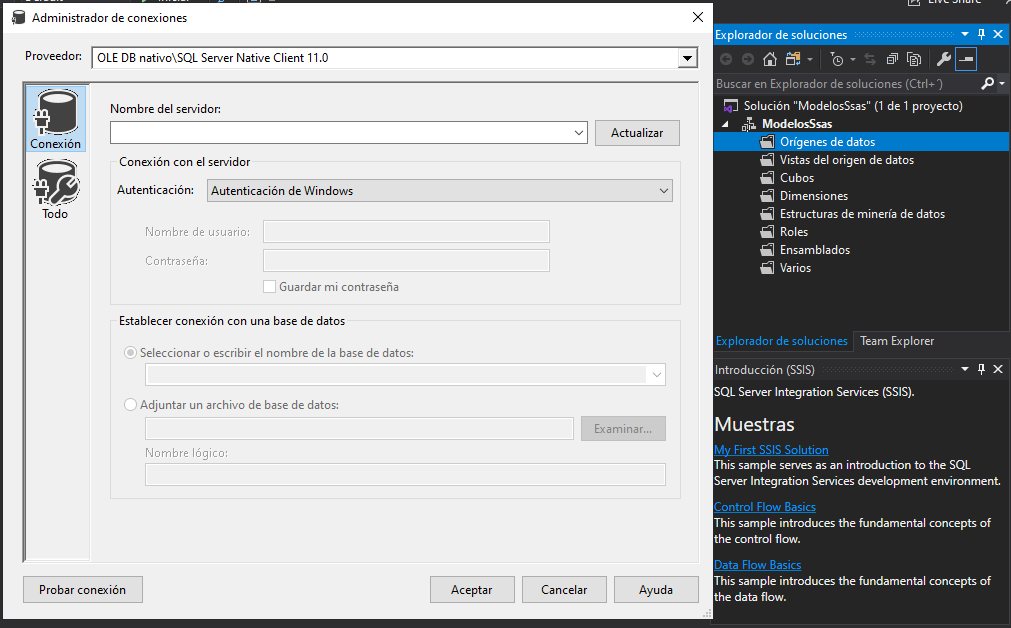
\includegraphics[width=\columnwidth]{images/task1/4}
    \end{center}	
    
Si todo está bien nos aparecerá la conexión creada en la sección de Data connections:
	\begin{center}
	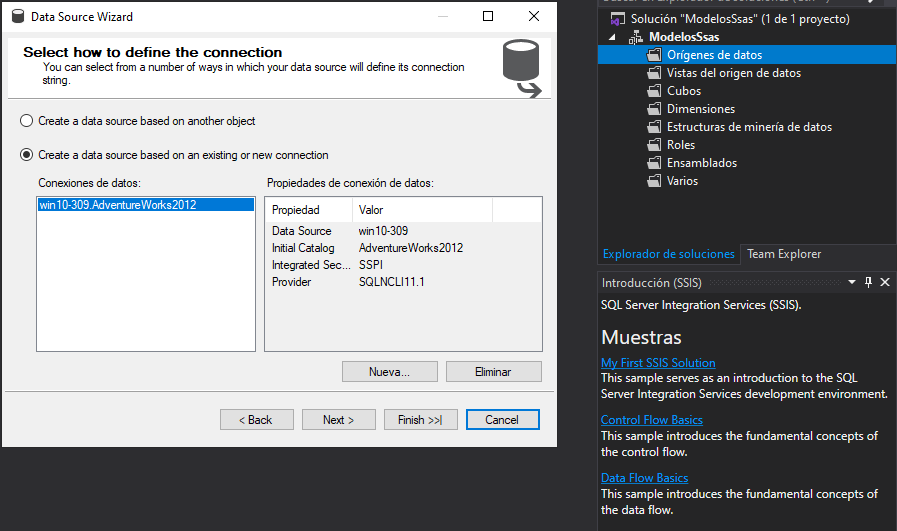
\includegraphics[width=\columnwidth]{images/task1/5}
    \end{center}	
    
En la ventana siguiente podemos definir las credenciales del Analysis Services y que utilizará para conectarse al Data Source. En este caso utilizaremos las mismas credenciales del servicio. Para eso elegimos Use the service account:
	\begin{center}
	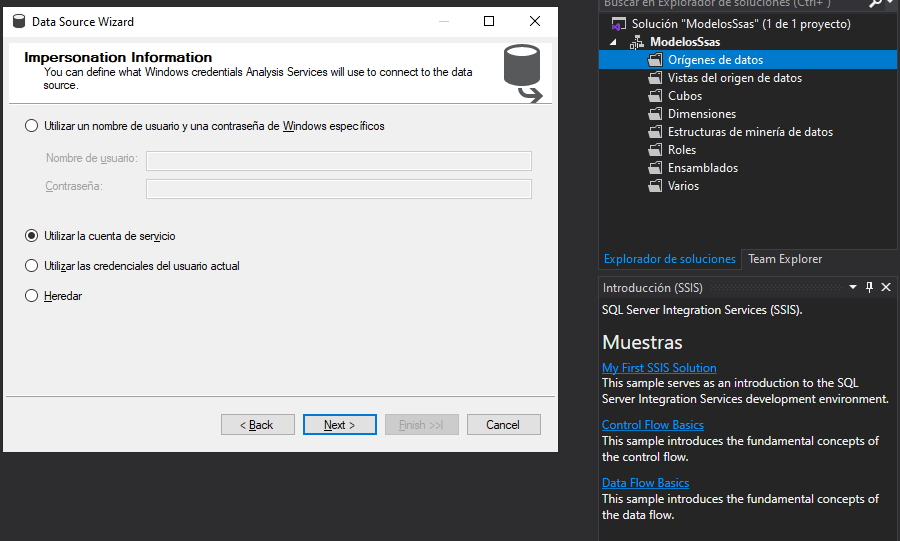
\includegraphics[width=\columnwidth]{images/task1/6}
    \end{center}	
    
	\begin{center}
	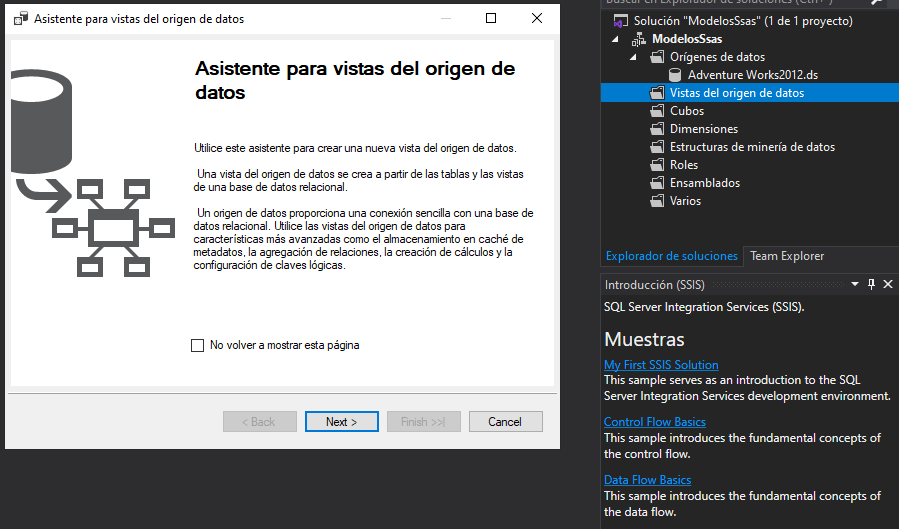
\includegraphics[width=\columnwidth]{images/task1/7}
    \end{center}	
Colocamos un nombre para el Data Source y click en Finish:
	\begin{center}
	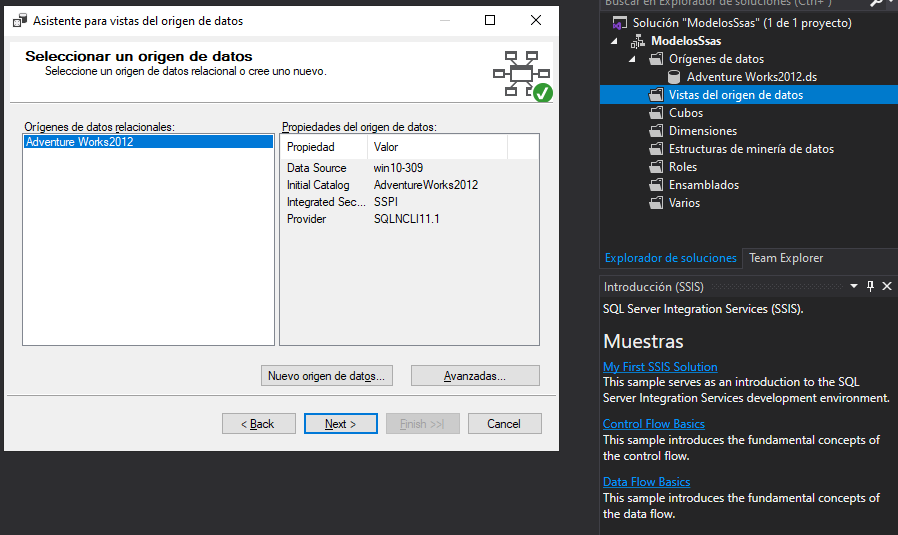
\includegraphics[width=\columnwidth]{images/task1/8}
    \end{center}	
